%!TEX TS-program = xelatex
%!TEX encoding = UTF-8 Unicode

\documentclass[11pt,a4paper,oneside]{book}
\usepackage[margin=2.5cm]{geometry}

% ------------------------------------------------------------------------------
% customize the headers with fancyhdr package
% ------------------------------------------------------------------------------
\usepackage{fancyhdr}
\fancyhf{}
\fancyhead[LE]{\leftmark}
\fancyhead[RO]{\nouppercase{\rightmark}}
\fancyfoot[LE,RO]{\thepage}
\pagestyle{fancy}

% ------------------------------------------------------------------------------
% Index
% ------------------------------------------------------------------------------
\usepackage{makeidx}
\makeindex

% ------------------------------------------------------------------------------
% Hyperlinks
% ------------------------------------------------------------------------------
\usepackage[colorlinks=true,linkcolor=blue]{hyperref}
\usepackage[all]{hypcap}  % Be sure to call this package after loading hyperref.

% ------------------------------------------------------------------------------
% Glossaries, must be after hyperref
% ------------------------------------------------------------------------------
% toc: add the glossaries to the table of contents.
% the glossaries to the table of contents.
% sort=standard is default, the other two are 'def' and 'use'.
\usepackage[xindy,toc,counter=section,style=listgroup]{glossaries}
% \usepackage[nogroupskip]{glossaries-extra}
\makeglossaries{}
% https://tex.stackexchange.com/questions/390201/glossaries-with-cjk-characters
% The approach, intended to sort by chinese and english, does not work
% \newrobustcmd{\cjkname}[1]{\begin{CJK}{UTF8}{min}#1\end{CJK}}
% \glsnoexpandfields
% \GlsXtrLoadResources[
%   src=dlbook-complete,% bib file
%   sort={cn-zh}% locale
%   dual-sort={en-GB},% locale used to sort secondary entries
%   type=chinese,% put the primary entries in the 'japanese' glossary
%   dual-type=english% put the dual entries in the 'english' glossary
% ]

% ------------------------------------------------------------------------------
% load tocbibind to add contents,list of figures, list of tables and
% bibliography into the toc
% ------------------------------------------------------------------------------
% \usepackage[utf8]{inputenc}
% \usepackage[english]{babel}
\usepackage[
	backend=bibtex,
	natbib,
	style=authoryear,
	citestyle=authoryear,
	maxbibnames=99,
	maxcitenames=1
]{biblatex}
\addbibresource{dlbook-complete.bib}

% make the 'et al.' italic
\DefineBibliographyStrings{english}{%
    andothers = {\it et\addabbrvspace al\adddot}
}

% A workaround to fix a known bug in biblatex, see http://tex.stackexchange.com/questions/311426/bibliography-error-use-of-blxbblverbaddi-doesnt-match-its-definition-ve
\makeatletter
\def\blx@maxline{77}
\makeatother

% \usepackage{natbib}
\usepackage{tocbibind}

% ------------------------------------------------------------------------------
% Needed to level up the bibliography in the toc
% ------------------------------------------------------------------------------
\usepackage{bookmark}

\usepackage[figurename=图.]{caption}

% ------------------------------------------------------------------------------
% Needed to load images
% ------------------------------------------------------------------------------
\usepackage{graphicx}
\graphicspath{{./figures/}}   % where to look for images

% ------------------------------------------------------------------------------
% for long and nice table
% ------------------------------------------------------------------------------
\usepackage{longtable}
\usepackage{booktabs}
\usepackage{ltxtable}

% for compact item list
\usepackage{paralist}
% \usepackage{enumitem}
\usepackage[inline]{enumitem}
% for algorithm
\usepackage[chapter]{algorithm}
\usepackage{algorithmic}
% \usepackage{algpseudocode}

% \renewcommand{\thealgorithm}{\arabic{chapter}.\arabic{algorithm}} 

% ------------------------------------------------------------------------------
% Math - Warning: before cjkfonts (xeCJK) and other package loads fontspec
% ------------------------------------------------------------------------------
\usepackage{amsmath}
\usepackage{amsfonts}
\usepackage{amssymb}
\numberwithin{equation}{chapter}

% font selection for mathematics with XeLaTeX, MUST after amsfonts
\usepackage{mathspec}
% \setmathsfont(Digits,Latin,Greek)[Numbers={Lining,Proportional}]{Minion Pro}

% There's no italic sans-serif math font by default, but it's needed in this book
% follow: http://tex.stackexchange.com/questions/77640/bold-italic-and-sans-serif-math-symbols
% to define a \mathsfit{} macro
\DeclareMathAlphabet{\mathsfit}{\encodingdefault}{\sfdefault}{m}{sl}
\SetMathAlphabet{\mathsfit}{bold}{\encodingdefault}{\sfdefault}{bx}{sl}

% ------------------------------------------------------------------------------
% Tikz
% ------------------------------------------------------------------------------

\usepackage{tikz}
\usetikzlibrary{calc,positioning,arrows.meta,shapes.geometric,shapes.misc }

% ------------------------------------------------------------------------------
% Localization setting
% ------------------------------------------------------------------------------

% load cjkfonts package and set Noto Sans SC as the default CJK fonts:
\usepackage[default,mdseries=Light,bfseries=Medium]{cjkfonts}

\usepackage{titlesec}

\titleformat{\part}[display]
{\centering\bfseries\Huge}%
{\Huge 第 \thepart{} 部分}%
{12 pt}%
{\bfseries\Huge}%

\titleformat{\chapter}[display]
  {\bfseries\huge}%
  {\huge 第 \thechapter{} 章}%
  {10 pt}%
  {\bfseries\huge}%

\renewcommand{\contentsname}{目录}
\renewcommand{\indexname}{索引}
\renewcommand{\figurename}{图}
\renewcommand{\tablename}{表}

% Redefine \emph to be both bold and italic, better in chinese document
%\let\emph\relax
%\DeclareTextFontCommand{\emph}{\bfseries\em} % bold and italic
%\DeclareTextFontCommand{\emph}{\bfseries} % just bold

\usepackage{indentfirst}

% ------------------------------------------------------------------------------
% Western fonts setting
% ------------------------------------------------------------------------------

% Set Roboto and Source Code Pro, which are installed with TexLive, for western
% fonts:

% \usepackage[no-math]{fontspec}

\newcommand{\robotodir}[0]{fonts/}
\newcommand{\sourcecodeprodir}[0]{fonts/}
\newcommand{\sourceserifprodir}[0]{fonts/}

\newcommand{\robotomd}[0]{Light}
\newcommand{\robotobf}[0]{Medium}
\newcommand{\robotoit}[0]{LightItalic}
\newcommand{\robotobi}[0]{MediumItalic}
\newcommand{\codepromd}[0]{Light}
\newcommand{\codeprobf}[0]{Medium}
\newcommand{\codeproit}[0]{LightIt}
\newcommand{\codeprobi}[0]{MediumIt}
\newcommand{\serifpromd}[0]{Light}
\newcommand{\serifprobf}[0]{Semibold}

\newfontfamily\Roboto{Roboto}[
  Extension=.ttf,
  Path=\robotodir,
  UprightFont=*-Regular,
  BoldFont=*-Bold,
  ItalicFont=*-Italic,
  BoldItalicFont=*-BoldItalic]

\newfontfamily\SourceCodePro{SourceCodePro}[
  Extension=.otf,
  Path=\sourcecodeprodir,
  UprightFont=*-\codepromd,
  BoldFont=*-\codeprobf,
  ItalicFont=*-\codeproit,
  BoldItalicFont=*-\codeprobi]

\newfontfamily\SourceSerifPro{SourceSerifPro}[
  Extension=.otf,
  Path=\sourceserifprodir,
  UprightFont=*-\serifpromd,
  BoldFont=*-\serifprobf]

\newcommand{\serif}[0]{\SourceSerifPro}

\newfontfamily\RobotoThin{Roboto}[
  Extension=.ttf,
  Path=\robotodir,
  UprightFont=*-Thin,
  ItalicFont=*-ThinItalic]

\newfontfamily\RobotoLight{Roboto}[
  Extension=.ttf,
  Path=\robotodir,
  UprightFont=*-Light,
  ItalicFont=*-LightItalic]

\newfontfamily\RobotoRegular{Roboto}[
  Extension=.ttf,
  Path=\robotodir,
  UprightFont=*-Regular,
  ItalicFont=*-Italic]

\newfontfamily\RobotoMedium{Roboto}[
  Extension=.ttf,
  Path=\robotodir,
  UprightFont=*-Medium,
  ItalicFont=*-MediumItalic]

\newfontfamily\RobotoBold{Roboto}[
  Extension=.ttf,
  Path=\robotodir,
  UprightFont=*-Bold,
  ItalicFont=*-BoldItalic]

\newfontfamily\RobotoBlack{Roboto}[
  Extension=.ttf,
  Path=\robotodir,
  UprightFont=*-Black,
  ItalicFont=*-BlackItalic]
  
\setmainfont{Roboto}[
  Extension=.ttf,
  Path=\robotodir,
  UprightFont=*-\robotomd,
  BoldFont=*-\robotobf,
  ItalicFont=*-\robotoit,
  BoldItalicFont=*-\robotobi]

\setsansfont{Roboto}[
  Extension=.ttf,
  Path=\robotodir,
  UprightFont=*-\robotomd,
  BoldFont=*-\robotobf,
  ItalicFont=*-\robotoit,
  BoldItalicFont=*-\robotobi]

\setmonofont{SourceCodePro}[
  Extension=.otf,
  Path=\sourcecodeprodir,
  UprightFont=*-\codepromd,
  BoldFont=*-\codeprobf,
  ItalicFont=*-\codeproit,
  BoldItalicFont=*-\codeprobi]

% ------------------------------------------------------------------------------
% Line space
% ------------------------------------------------------------------------------
\usepackage{setspace}
\onehalfspacing{}

%sierxue添加
%\usepackage{marginnote}

%sierxue添加
\newtheorem{theorem}{Theorem}
\newtheorem{corollary}[theorem]{Corollary}
\newtheorem{lemma}[theorem]{Lemma}
\newtheorem{observation}[theorem]{Observation}
\newtheorem{proposition}[theorem]{Proposition}
\newtheorem{definition}[theorem]{Definition}
\newtheorem{claim}[theorem]{Claim}
\newtheorem{fact}[theorem]{Fact}
\newtheorem{assumption}[theorem]{Assumption}

%------------------------------定理名称中文化-----------------------------%
\newtheorem{dingyi}{\textbf 定义~}[section]
\newtheorem{dingli}{\textbf 定理~}[section]
\newtheorem{yinli}[dingli]{\textbf 引理~}
\newtheorem{tuilun}[dingli]{\textbf 推论~}
\newtheorem{mingti}[dingli]{\textbf 命题~}
\newtheorem{lizi}{{例}}%sierxue

%sierxue添加自定义命令
%\newcommand{\vocab}[1]{\emph{#1}} %vocab words
%\newcommand{\vocabaka}[2]{\vocab{#1}(a.k.a. #2)} %vocab words with synonyms
\newcommand{\cndot}[1]{{\ahei \CJKunderdot{#1}}}

% ------------------------------------------------------------------------------
% Load glossaries
% ------------------------------------------------------------------------------
%% glossaries

% ganx ml

\newglossaryentry{ml}{
  name={机器学习},
  description={\emph{Machine learning}},
  sort={jqxx}
}

\newglossaryentry{feature}{
  name={特征},
  description={\emph{Feature}},
  sort={tz}
}

\newglossaryentry{feature2}{
  name={Feature},
  description={特征},
}

\newglossaryentry{norm}{
  name={范数},
  description={norm}
}

\newglossaryentry{dl}{
  name={深度学习},
  description={\emph{Deep Learning}}
}


% ------------------------------------------------------------------------------
% The document body
% ------------------------------------------------------------------------------

\begin{document}

% file: title.tex

\begin{titlepage}
\begin{center}
  \hfill\\
  \vspace{1cm}
  % title of this document
  {\fontsize{36pt}{40pt}\NotoSansSCBold{} 深度学习}\\
  \vspace{1em}
  {\LARGE\serif \href{http://www.deeplearningbook.org/}{Deep Learning}}\\
  \vspace{1cm}
  %\includegraphics{cayley}\\
  \vspace{1cm}
  
  {\large\serif
  \begin{tabular}{c}
    Ian Goodfellow \\
    Yoshua Bengio \\
    Aaron Courville
  \end{tabular}
  }
   
  \vfill
  {\large \today}\\
  \vspace{1em}
  {\large Draft}
\end{center}
\end{titlepage}


\frontmatter

%\maketitle

\tableofcontents
%\listoffigures
%\listoftables

\pagebreak

% file: author.tex

\chapter{关于作者}
\label{ch:Author}

\begin{minipage}{0.7\linewidth}
\textbf{甘湘华}

你可以在其主页 \href{http://sierxue.me/about}{作者主页} 了解更多信息。
\end{minipage}
\hfill
\begin{minipage}{0.25\linewidth}
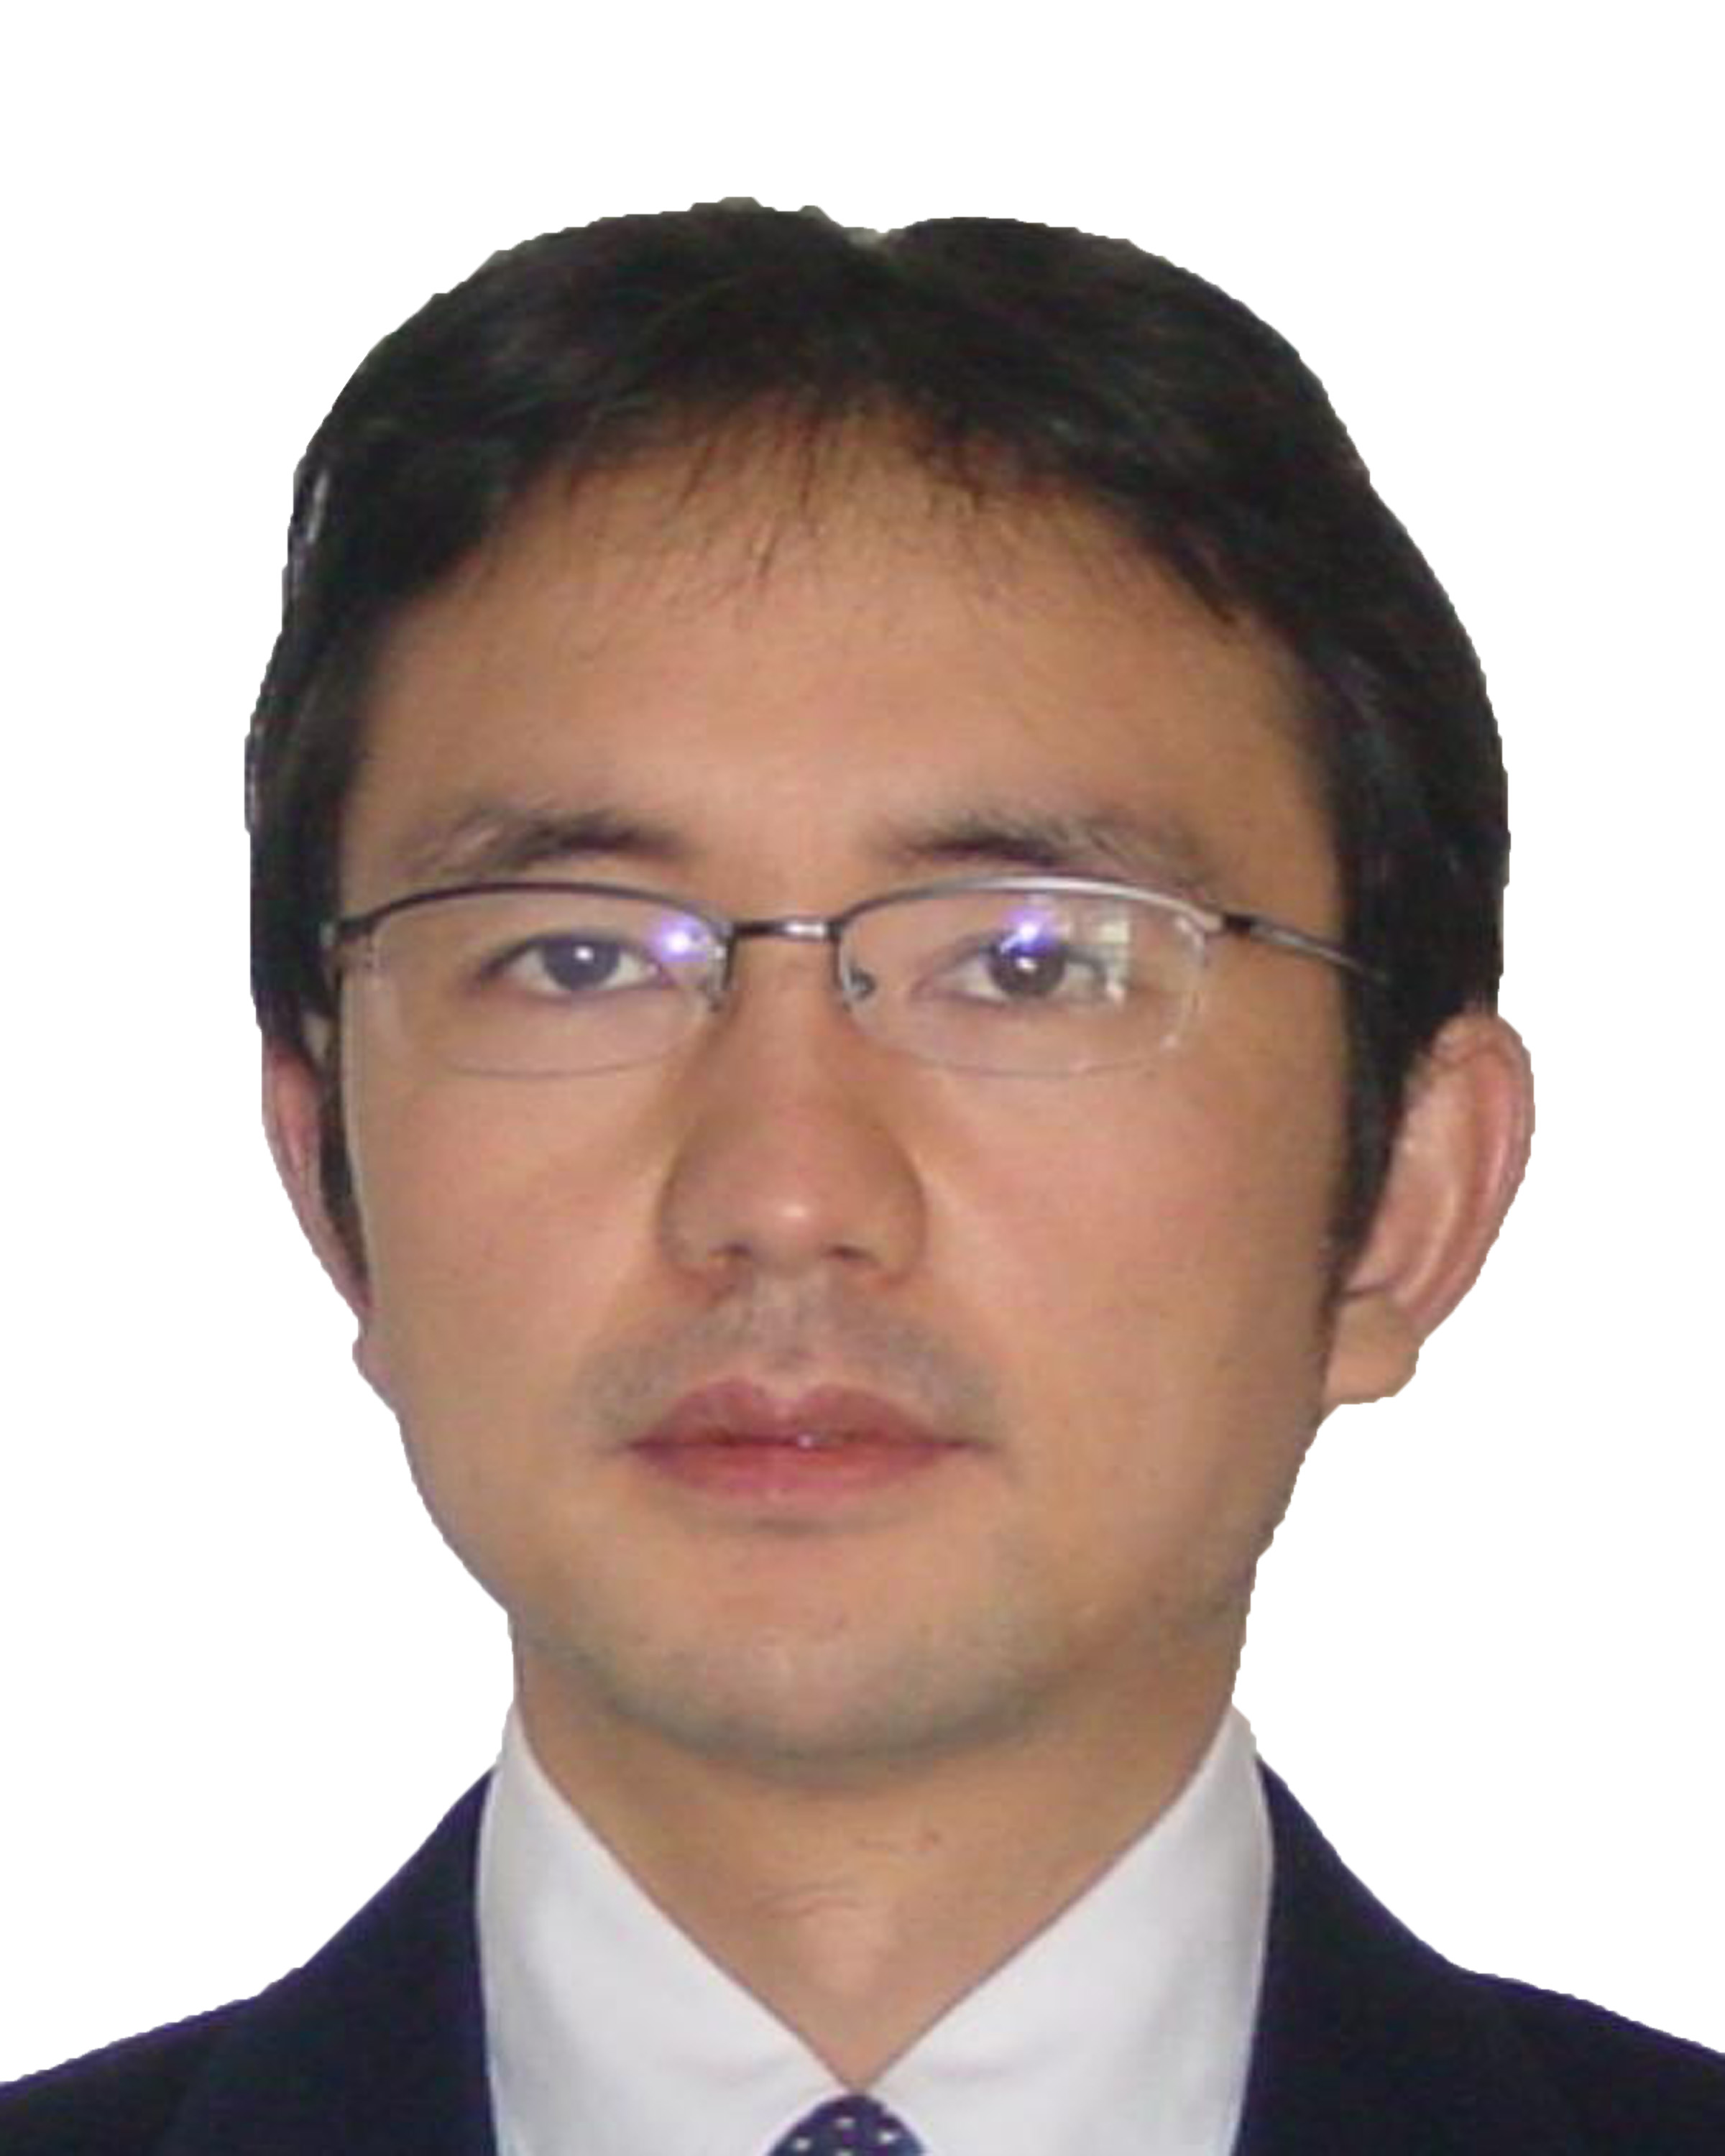
\includegraphics[width=\textwidth]{Gan_author_image.jpg}  
\end{minipage}

\chapter{致谢}
\label{ch:Acknowledgements}

没有许多人的贡献,本书是不可能完成的。

\chapter{数学符号}
\label{ch:notation}

这一部分提供了一个简明的索引,描述整本书中使用的数学符号。如果你不熟悉任何对应的
数学概念,这个符号索引可能看起来很吓人。然而,不要绝望,我们在 2 --- 4 章里描述了
这些概念的大部分。

\begin{center}
  \setstretch{1.5}
  {\Large\bfseries 数和数组}\\
  \vspace{1em}
  \begin{tabular}{c l}
    $a$ & 标量(整数或实数)\\
    $\pmb{a}$ & 向量 \\
    $\pmb{A}$ & 矩阵 \\
    $\pmb{\mathsf{A}}$ & 张量 \\
    $\pmb{I}_n$ & $n$ 行 $n$ 列的单位矩阵 \\
    $\pmb{I}$ & 单位矩阵,其维度隐含在上下文中 \\
    $\pmb{e}^{(i)}$ & 标准的基向量 $[0, \ldots, 0, 1, 0, \ldots, 0]$,$1$ 的位置由 $i$ 确定 \\
    $\mathrm{diag}(\pmb{a})$ & 对角线元素为 $\pmb{a}$ 的对角矩阵 \\
    $\mathrm{a}$ & 标量随机变量 \\
    $\mathbf{a}$ & 向量值随机变量 \\
    $\mathbf{A}$ & 矩阵值随机变量
  \end{tabular}
\end{center}

\vspace{1em}

\begin{center}
  \setstretch{1.5}
  {\Large\bfseries 集合和图}\\
  \vspace{1em}
  \begin{tabular}{c l}
    $\mathbb{A}$ & 集合 \\
    $\mathbb{R}$ & 实数集合 \\
    $\{0,1\}$ & 包含 $0$ 和 $1$ 的集合 \\
    $\{0,1,\ldots,n\}$ & $0$ 到 $n$ 的所有整数集合 \\
    $[a,b]$ & 包括 $a$ 和 $b$ 的实数区间 \\
    $(a,b]$ & 左开右闭区间,不包括 $a$ 但包括 $b$ \\
    $\mathbb{A}\backslash\mathbb{B}$ & 集合差,例如,包含有 $\mathbb{A}$ 的元素但其不在 $\mathbb{B}$ 中的集合 \\
    $\mathcal{G}$ & 图 \\
    $Pa_{\mathcal{G}}(x_i)$ & 图  $\mathcal{G}$ 中 $x_i$ 的父顶点
  \end{tabular}
\end{center}

\vspace{1em}

\begin{center}
  \setstretch{1.5}
  {\Large\bfseries 索引}\\
  \vspace{1em}
  \begin{tabular}{c l}
    $a_i$ & 向量 $\pmb{a}$ 的第 $i$ 个元素,索引起始位置为 $1$ \\
    $a_{-i}$ & 向量 $\pmb{a}$ 中除了第 $i$ 个元素之外的所有其它元素 \\
    $A_{i,j}$ & 矩阵 $\pmb{A}$ 的 $i,j$ 位置元素 \\
    $A_{i,:}$ & 矩阵 $\pmb{A}$ 的第 $i$ 行 \\
    $A_{:,i}$ & 矩阵 $\pmb{A}$ 的第 $i$ 列 \\
    $\mathsfit{A}_{i,j,k}$ & 三维张量 $\pmb{\mathsf{A}}$ 的 $(i,j,k)$ 位置的元素 \\
    $\pmb{\mathsf{A}}_{:,:,i}$ & 三维张量在 $i$ 处的二维切分 \\
    $\mathrm{a}_i$ & 随机向量 $\mathbf{a}$ 的第 $i$ 个元素
  \end{tabular}
\end{center}

\vspace{1em}

\begin{center}
  \setstretch{1.5}
  {\Large\bfseries 线性代数操作}\\
  \vspace{1em}
  \begin{tabular}{c l}
    $\pmb{A}^{\top}$ & 矩阵 $\pmb{A}$ 的转置 \\
    $\pmb{A}^+$ & 矩阵 $\pmb{A}$ 的摩尔--彭若斯广义逆 \\
    $\pmb{A} \odot \pmb{B}$ & 矩阵 $\pmb{A}$ 和 $\pmb{B}$ 的按元素(阿达玛)乘积 \\
    $\det(\pmb{A})$ & 矩阵 $\pmb{A}$ 的行列式
  \end{tabular}
\end{center}

\vspace{1em}

\begin{center}
  \setstretch{1.5}
  {\Large\bfseries 微积分}\\
  \vspace{1em}
  \begin{tabular}{c l}
    $\frac{dy}{dx}$ & $y$ 对 $x$ 求导 \\
    $\frac{\partial y}{\partial x}$ & $y$ 对 $x$ 求偏微分 \\
    $\nabla_{\pmb{x}}y$ & $y$ 在 $\pmb{x}$ 上的梯度 \\
    $\nabla_{\pmb{X}}y$ & $y$ 对 $\pmb{X}$ 求矩阵导数 \\
    $\nabla_{\pmb{\mathsf{X}}}y$ & 包含 $y$ 对 $\pmb{\mathsf{X}}$ 求得的导数的张量 \\
    $\frac{\partial f}{\partial \pmb{x}}$ & $f : \mathbb{R}^n \rightarrow \mathbb{R}^m$ 的雅可比矩阵 $\pmb{J} \in \mathbb{R}^{m \times n}$ \\
    $\nabla^2_{\pmb{x}}f(\pmb{x})$ 或 $\pmb{H}(f)(\pmb{x})$ & $f$ 在输入点 $\pmb{x}$ 的海森矩阵\\
    $\displaystyle\int f(\pmb{x})d\pmb{x}$ & 在整个 $\pmb{x}$ 上的定积分\\
    $\displaystyle\int_{\mathbb{S}} f(\pmb{x})d\pmb{x}$ & 在集合 $\mathbb{S}$ 上对 $\pmb{x}$ 的定积分 \\
  \end{tabular}
\end{center}

\vspace{1em}

\begin{center}
  \setstretch{1.5}
  {\Large\bfseries 概率与信息论}\\
  \vspace{1em}
  \begin{tabular}{c l}
    $\mathrm{a} \bot \mathrm{b}$ & 随机变量 $\mathrm{a}$ 与 $\mathrm{b}$ 互相独立 \\
    $\mathrm{a} \bot \mathrm{b}\: | \: \mathrm{c}$ & 给定 $\mathrm{c}$ 时它们条件独立 \\
    $P(\mathrm{a})$ & 一个离散变量上的概率分布 \\
    $p(\mathrm{a})$ & 一个连续变量,或者类型没有指定的变量上的概率分布 \\
    $\mathrm{a} \sim P$ & 随机变量 $\mathrm{a}$ 具有 $P$ 的分布 \\
    $\mathbb{E}_{\mathrm{x} \sim P} [f(x)]$ 或 $\mathbb{E}f(x)$ & $f(x)$ 对 $P(\mathrm{x})$ 的期望 \\
    $\mathrm{Var}(f(x))$ & 在 $P(\mathrm{x})$ 下 $f(x)$ 的方差 \\
    $\mathrm{Cov}(f(x),g(x))$ & 在 $P(\mathrm{x})$ 下 $f(x)$ 和 $g(x)$ 的协方差 \\
    $H(\mathrm{x})$ & 随机变量 $\mathrm{x}$ 的香农熵 \\
    $D_{\mathrm{KL}}(P \parallel Q)$ & $\mathrm{P}$ 和 $\mathrm{Q}$ 的 $\mathrm{KL}$ 散度 \\
    $\mathcal{N}(\pmb{x};\pmb{\mu};\pmb{\Sigma})$ & $\pmb{x}$ 上均值为 $\pmb{\mu}$,协方差为 $\pmb{\Sigma}$ 的高斯分布 \\
  \end{tabular}
\end{center}

\vspace{1em}

\begin{center}
  \setstretch{1.5}
  {\Large\bfseries 函数}\\
  \vspace{1em}
  \begin{tabular}{c l}
    $f : \mathbb{A} \rightarrow \mathbb{B}$ & 定义域为 $\mathbb{A}$,值域为 $\mathbb{B}$ 的函数 $f$ \\
    $f \circ g$ & 函数 $f$ 和 $g$ 的组合 \\ % 复合函数
    $f(\pmb{x};\pmb{\theta})$ & $\pmb{x}$ 的函数,$\pmb{x}$ 由 $\pmb{\theta}$ 参数化。有时候我们只写 $f(\pmb{x})$,忽略参数 $\pmb{\theta}$ 来简化符号。 \\
    $\log x$ & $x$ 的自然对数 \\
    $\sigma(x)$ & {\serif Logistic sigmoid},$\displaystyle\frac{1}{1 + \exp(-x)}$ \\
    $\zeta(x)$ & {\serif Softplus},$\log(1 + \exp(x))$ \\
    $||\pmb{x}||_p$ & $\pmb{x}$ 的 $L^p$ 范数 \\
    $||\pmb{x}||$ & $\pmb{x}$ 的 $L^2$ 范数 \\
    $x^+$ & $x$ 的正数部分,即 $\max(0,x)$ \\
    $\pmb{1}_{\mathrm{condition}}$ & 如果条件真为 $1$,否则为 $0$ \\
  \end{tabular}
\end{center}

有时候我们使用一个参数是一个标量的函数 $f$,但是将它应用到一个向量、矩阵或者张量:
$f(\pmb{x})$,$f(\pmb{X})$,或 $f(\pmb{\mathsf{X}})$。这意思是将 $f$ 按元素应用
到数组。例如,如果 $\pmb{\mathsf{C}} = \sigma(\pmb{\mathsf{X}})$,那么对于所有有
效的 $i$,$j$ 和 $k$ 的值,$\mathsfit{C}_{i,j,k} = \sigma(\mathsfit{X}_{i,j,k})$。

\vspace{1em}

\begin{center}
  \setstretch{1.5}
  {\Large\bfseries 数据集和分布}\\
  \vspace{1em}
  \begin{tabular}{c l}
    $p_{\mathrm{data}}$ & 数据生成的分布 \\
    $\hat{p}_{\mathrm{data}}$ & 由训练集定义的经验分布 \\
    $\mathbb{X}$ & 一个训练样本集 \\
    $\pmb{x}^{(i)}$ & (输入自)数据集的第 $i$ 个样本 \\
    $y^{(i)}$ 或 $\pmb{y}^{(i)}$ & 与 $\pmb{x}^{(i)}$ 关联的有监督学习的目标 \\
    $\pmb{X}$ & $m \times n$ 矩阵,其具有在 $\pmb{X}_i$ 行中的输入样本 $\pmb{x}^{(i)}$ \\
    % TODO: 原文最后有个冒号,可能还没完成
  \end{tabular}
\end{center}


\mainmatter{}

% intro.tex

\chapter{介绍}
\label{ch:intro}

长久以来,发明家们梦想着创造会思考的机器。
当可编程计算机最初被设想时~——~在它被建造的超过一百年前~——~人们就想知道
它们是否可能变得智能\citep{Lovelace1842}。

% file: chap2.tex

\chapter{一个温柔的开始}
\label{ch:aGentleStart}

\begin{lizi}
  {\large \akai 预测木瓜是否味美:}
  \upshape {想象一下你刚刚抵达太平洋小岛,
你很快发现木瓜是当地饮食的一个重要组成部分。
但是,你从来没有尝过木瓜。你想通过学习去预测你在市场上看到的木瓜是否可口。
首先,你需要决定你的预测应该基于木瓜的什么\textbf{\gls{feature}}
(\gls{feature2})。
根据你以前吃水果形成的经验,你决定使用两个特征:木瓜的颜色和木瓜的柔软度。
作为\textbf{学习者}
(learner)的你,可以随机地抽取一些木瓜作为\textbf{训练样本} (training
sample), 记录下每一个木瓜的颜色和柔软度,然后试吃以判定木瓜是否美味。
根据这些数据,你可以生成一个\textbf{预测规则} (prediction rule)。
我们的第一步,是建立一个数学模型来刻画这样的学习问题。}
\end{lizi}

\section{一个统计学习的数学模型}

\subsection{统计学习框架:}

这个统计框架 (statistical learning framework)包含四部分: \textbf{输入}
(input)、\textbf{输出} (output)、\textbf{数据生成模型} (data-generation
model)、 以及\textbf{成效} (measure of success)。

\subsubsection{学习者的输入}

\begin{enumerate}

\item
  \textbf{样本空间} (domain space, or domain set, or instance space):
  一个任意的集合,通常表示为\(\mathcal{X}\),它是我们想要研究的对象的集合。
  在上面的例子中,\(\mathcal{X}\)就是所有的木瓜的集合。
  通常\(\mathcal{X}\)中的一个\textbf{样本}
  (sample),通常表示为一个小写的\(x\), 可以由一个\textbf{特征向量}
  (feature vector)来表示,比如木瓜的颜色和柔软度。
  如果用一个值表示颜色,一个值表示柔软度,那么\(x\)可以用一个二元数组来表示。
  我们也称一个样本为一个\textbf{示例}
  (instance),\(\mathcal{X}\)为\textbf{示例空间} (instance space)。
\item
  \textbf{标记空间} (label space or label
  set):通常表示为\(\mathcal{Y}\)。
  对于本例,\(\mathcal{Y}\)为二值集合,通常表示为\(\{0,1\}\):1代表味美,0代表非味美。
\item
  \textbf{训练数据} (training data):通常表示为
  \[S = \left(\left(x_1,y_1\right),\ldots,\left(x_m,y_m\right)\right)\]
  其中,\(x_i\),
  \(i=1,\ldots,m\),为第\(i\)个样本,\(y_i\)为对第\(i\)个样本所做的标记。
  我们称\(\left(x_i,y_i\right)\)为第\(i\)个\textbf{样例}(example)。
  简单地说,训练数据就是一组使按顺序排列的样例。\footnote{示例和样例的区别是什么,他们对应的英文单词分别是什么?}
\end{enumerate}

\subsubsection{学习者的输出}

通过对样例的学习,学习者输出一个预测准则,\[h: \mathcal{X} \rightarrow \mathcal{Y}\]。
我们称这个函数为一个\textbf{预测器} (predictor),或是\textbf{假设}
(hypothesis),或是\textbf{分类器} (classifier)。
这个预测器可以用来标记新样本。在本例中,预测器可以用来标记市场上的木瓜是否味美。
根据训练数据,学习者可以构造某种学习算法来得到一个预测器。

\subsubsection{数据生成模型}

首先,我们假定样本来自于某个概率分布\(\mathcal{D}\)。
在本例中,学习者对\(\mathcal{D}\)\emph{一无所知},并且\(\mathcal{D}\)可以是任意的概率分布。
在本例中,我们假设有一个``正确''的预测器\(f\)。
预测器\(f\)对于学习者来说也是未知的。事实上,学习者梦寐以求的正是这个预测器。
总的说来,\(S\)中的任意一个样例\(\left(x_i,y_i\right)\)是这样产生的:

\begin{enumerate}

\item
  按照\(\mathcal{D}\)抽样产生一个样本\(x_i\);
\item
  用正确的预测器来标记\(x_i\),即\(y_i=f(x_i)\).
\end{enumerate}

\subsubsection{成效}

学习者通过对训练数据的学习,生成一个预测器\(h\)后,怎么来评判这个预测器的好坏呢?
一个顺理成章的标准是判断这个预测器犯错误的概率的大小。数学上,我们可以表示为:
\[
\begin{aligned}
L_{\mathcal{D},f}(h) \overset{\underset{\mathrm{def}}{}}{=} \mathbb P_{x \sim D}\left[h(x) \neq f(x)\right] \overset{\underset{\mathrm{def}}{}}{=} \mathcal{D}\left(\left\{x:h(x) \neq f(x)\right\}\right)
\end{aligned}
\] 我们称\(L_{\mathcal{D},f}(h)\)为\textbf{预测错误} (error of a
predictor 或者 error of a classifier 或者 generalization error 或者 risk
或者 true error)。 注意\(L_{\mathcal{D},f}(h)\)中的下标
\(\mathcal{D},f\) 表示这个预测错误的度量 (measure)
是基于样本分布\(\mathcal{D}\)及正确的预测器\(f\)。 如果上下文的语境中
\(\mathcal{D},f\) 很清楚的话,我们有时为简洁的缘故会省略掉下标。

\subsubsection{思考和练习}

\begin{enumerate}

\item
  在本例中,输入、输出、和数据生成模型分别是什么?
\item
  学习者所拥有的信息是什么?\footnote{简单说来,学习者所有信息就是训练数据\(S\)。在本例中,最初,学习者不知道木瓜颜色和柔软度的概率分布,也不知道具有某种颜色和某种柔软度的木瓜口味如何。学习者对木瓜的了解来源于\(S\)。}
\end{enumerate}

% file: part_basics.tex
% source: http://www.deeplearningbook.org/contents/part_basics.html

\part{应用于本书的数学和机器学习基础}
\label{part_basics}

本书的这一部分介绍理解\gls*{dl}所需要的基本的数学概念。
我们从应用于本书的数学的 一般概念开始,这些数学允许我们定义多元函数,
找到这些函数的最高和最低点,并量化置信度。

接下来,我们描述\gls*{ml}的基本目标。我们描述如何通过指定一个代表某些置信度的模
型来完成这些目标,设计一个衡量这些置信度与现实有多符合的代价函数,并用一个训练算
法来最小化那个代价函数。

这个基本框架是各种各样\gls*{ml}算法的基础,包括非深度\gls*{ml}的方法。在本书随后
部分中,我们在这个框架内开发\gls*{dl}算法。

% \input{contents/linear_algebra}
% \input{contents/prob}
% \input{contents/numerical}
% \input{contents/ml}
% \input{contents/part_practical}
% \input{contents/mlp}
% \input{contents/regularization}
% \input{contents/optimization}
% \input{contents/convnets}
% \input{contents/rnn}
% \input{contents/guidelines}
% \input{contents/applications}
% \input{contents/part_research}
% \input{contents/linear_factors}
% \input{contents/autoencoders}
% \input{contents/representation}
% \input{contents/graphical_models}
% \input{contents/monte_carlo}
% \input{contents/partition}
% \input{contents/inference}
% \input{contents/generative_models}

% \appendix
% appendix chapters here

\backmatter{}

\bookmarksetup{startatroot}

\printbibliography[
	heading=bibintoc,
	title={参考文献}
]
\printindex
\printglossary[title={术语表}]

\end{document}
